\chapter{Experimental Results and Visualization}
\label{chap:results}

This chapter presents the empirical results captured from $1\,680$ search trials and $1\,080$ sorting trials, incorporating all nine publication-quality figures and structured LaTeX summary tables.

\section{Mathematical Growth Functions}
Figures \ref{fig:growth_common} and \ref{fig:growth_hierarchy} (in Chapter \ref{chap:growth}) established the theoretical curves. As shown in Table \ref{tab:growth_functions}, factorial and exponential functions diverge astronomically, whereas logarithmic and linear functions remain exceptionally well-behaved across orders of magnitude.

\section{Searching Algorithms Empirical Results}
Table \ref{tab:search_worst_summary} presents the worst-case experimental measurements for Linear Search and Binary Search when the target key is absent from the sequence.

\begin{table}[htbp]
\centering
\caption{Searching Algorithms Worst-Case Empirical Telemetry (Missing Target)}
\label{tab:search_worst_summary}
\small
\begin{tabular*}{\textwidth}{@{\extracolsep{\fill}}lrrrrrr}
\toprule
\textbf{Algorithm} & $n$ & \textbf{Key Comps} & \textbf{Median ($\mu$s)} & \textbf{Mean ($\mu$s)} & \textbf{Std Dev ($\mu$s)} & \textbf{IQR ($\mu$s)} \\
\midrule
Binary Search & 100 & 14 & 0.69 & 0.69 & 0.02 & 0.01 \\
Linear Search & 100 & 100 & 3.33 & 3.31 & 0.08 & 0.15 \\
Binary Search & 500 & 18 & 1.08 & 1.09 & 0.02 & 0.01 \\
Linear Search & 500 & 500 & 18.50 & 18.42 & 0.17 & 0.20 \\
Binary Search & 1000 & 20 & 1.19 & 1.20 & 0.05 & 0.02 \\
Linear Search & 1000 & 1000 & 37.95 & 38.32 & 1.08 & 0.57 \\
Binary Search & 5000 & 26 & 1.50 & 1.51 & 0.03 & 0.02 \\
Linear Search & 5000 & 5000 & 197.15 & 197.78 & 2.77 & 2.70 \\
Binary Search & 10000 & 28 & 1.63 & 1.64 & 0.04 & 0.04 \\
Linear Search & 10000 & 10000 & 382.05 & 381.96 & 5.86 & 7.42 \\
Binary Search & 50000 & 32 & 1.85 & 1.85 & 0.05 & 0.09 \\
Linear Search & 50000 & 50000 & 1922.25 & 1925.47 & 28.43 & 39.92 \\
Binary Search & 100000 & 34 & 1.96 & 1.98 & 0.05 & 0.01 \\
Linear Search & 100000 & 100000 & 3822.10 & 3882.46 & 236.84 & 97.40 \\
\bottomrule
\end{tabular*}
\end{table}


\subsection{Comparison of Searching Operation Counts}
Figure \ref{fig:search_ops} illustrates key comparisons across input sizes and target locations.

\begin{figure}[htbp]
    \centering
    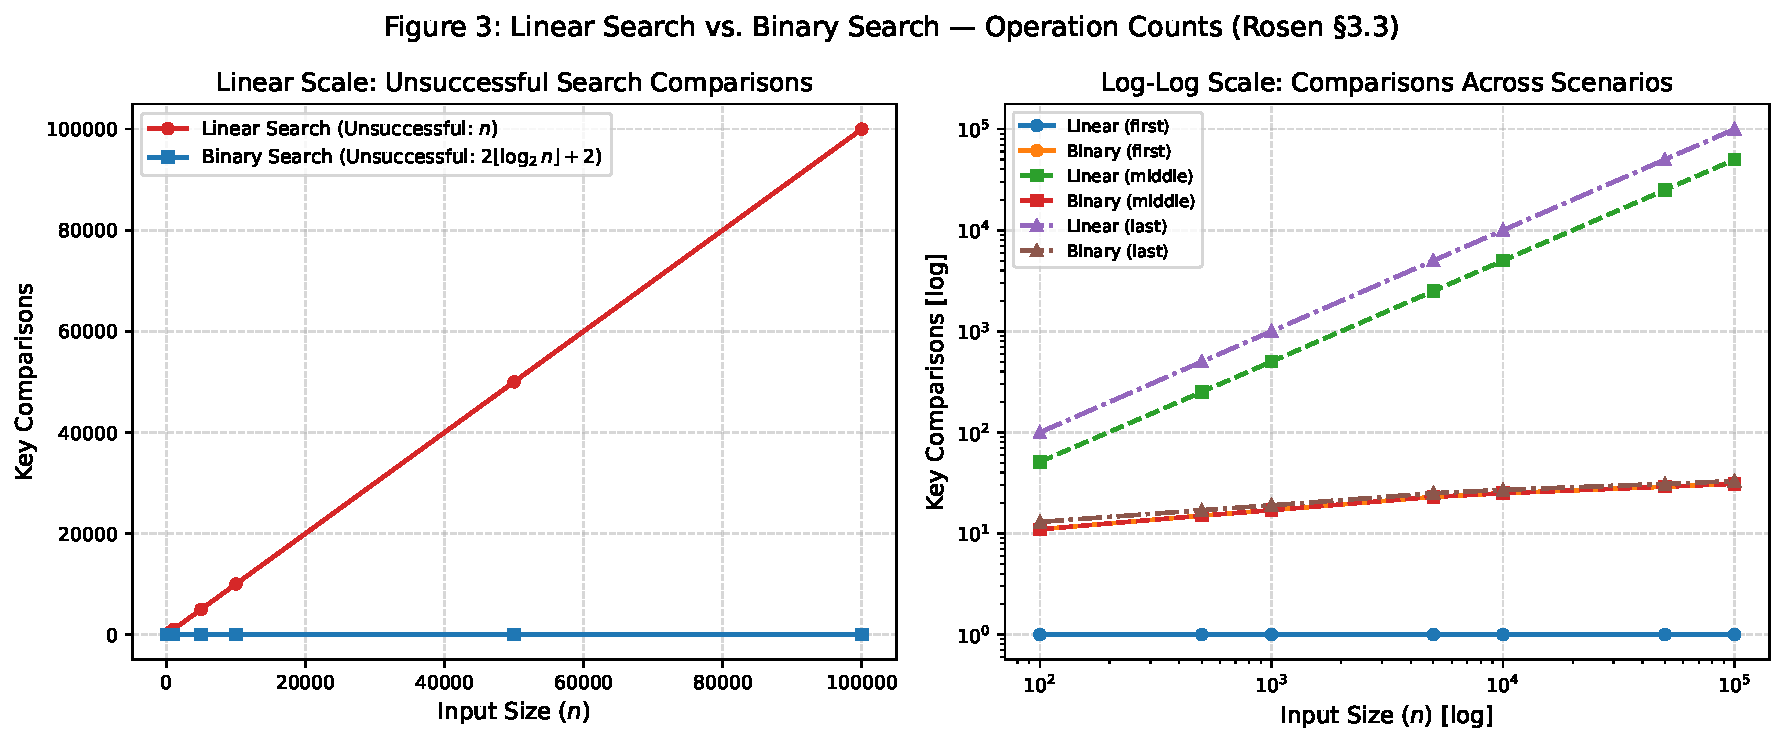
\includegraphics[width=0.95\textwidth]{latex/figures/figure3_search_operation_counts.pdf}
    \caption{Figure 3: Linear Search vs. Binary Search — Operation Counts (Rosen §3.3).}
    \label{fig:search_ops}
\end{figure}

Notice in the left linear plot of Figure \ref{fig:search_ops} that Linear Search comparisons grow on a steep line $T(n) = n$, reaching $100\,000$ comparisons at $n = 100\,000$. In stark contrast, Binary Search comparisons appear as a flat line hugging the horizontal axis, reaching only $34$ comparisons at $n = 100\,000$. In the right log-log plot, the power-law slope of Linear Search is $1.0$, while Binary Search exhibits logarithmic scaling.

\subsection{Comparison of Searching Execution Times}
Figure \ref{fig:search_times} depicts median execution times with error bars denoting $\pm 1$ standard deviation.

\begin{figure}[htbp]
    \centering
    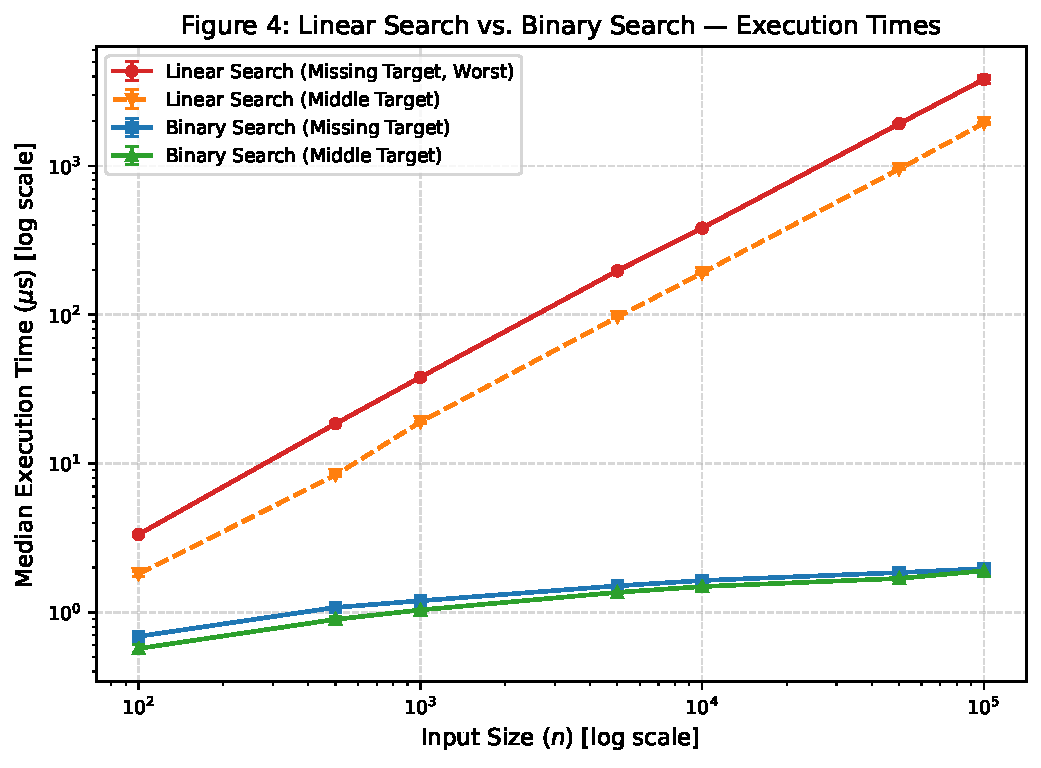
\includegraphics[width=0.88\textwidth]{latex/figures/figure4_search_execution_times.pdf}
    \caption{Figure 4: Linear Search vs. Binary Search — Execution Times on Log-Log Scale.}
    \label{fig:search_times}
\end{figure}

At $n = 100\,000$ (missing target), Linear Search requires a median duration of $3\,820.0\,\mu\text{s}$ ($3.82\text{ ms}$), while Binary Search requires only $1.96\,\mu\text{s}$—an empirical speedup of $\approx 1\,946\times$.

\section{Sorting Algorithms Empirical Results}
Table \ref{tab:sorting_random_summary} presents the empirical measurements for Bubble Sort and Insertion Sort operating on random permutations of distinct integers.

\begin{table}[htbp]
\centering
\caption{Sorting Algorithms Empirical Telemetry on Random Permutations}
\label{tab:sorting_random_summary}
\small
\begin{tabular*}{\textwidth}{@{\extracolsep{\fill}}lrrrrrr}
\toprule
\textbf{Algorithm} & $n$ & \textbf{Comparisons} & \textbf{Swaps / Shifts} & \textbf{Median (ms)} & \textbf{Mean (ms)} & \textbf{Std Dev (ms)} \\
\midrule
Bubble Sort & 100 & 4,950 & 2,502 & 0.38 & 0.38 & 0.01 \\
Insertion Sort & 100 & 2,597 & 2,502 & 0.19 & 0.19 & 0.01 \\
Bubble Sort & 250 & 31,125 & 15,618 & 2.29 & 2.29 & 0.02 \\
Insertion Sort & 250 & 15,863 & 15,618 & 1.13 & 1.13 & 0.02 \\
Bubble Sort & 500 & 124,750 & 61,188 & 9.57 & 9.58 & 0.13 \\
Insertion Sort & 500 & 61,682 & 61,188 & 4.76 & 4.74 & 0.07 \\
Bubble Sort & 1000 & 499,500 & 248,445 & 42.78 & 42.72 & 0.46 \\
Insertion Sort & 1000 & 249,438 & 248,445 & 20.23 & 20.30 & 0.33 \\
Bubble Sort & 2000 & 1,999,000 & 1,026,195 & 176.56 & 177.16 & 2.41 \\
Insertion Sort & 2000 & 1,028,183 & 1,026,195 & 85.42 & 86.30 & 3.51 \\
Bubble Sort & 3000 & 4,498,500 & 2,296,691 & 405.59 & 406.85 & 6.62 \\
Insertion Sort & 3000 & 2,299,685 & 2,296,691 & 191.65 & 191.80 & 3.41 \\
\bottomrule
\end{tabular*}
\end{table}


\subsection{Sorting Operation Counts: Comparisons and Data Movements}
Figure \ref{fig:sorting_ops} contrasts element comparisons and data movement operations (swaps versus right shifts).

\begin{figure}[htbp]
    \centering
    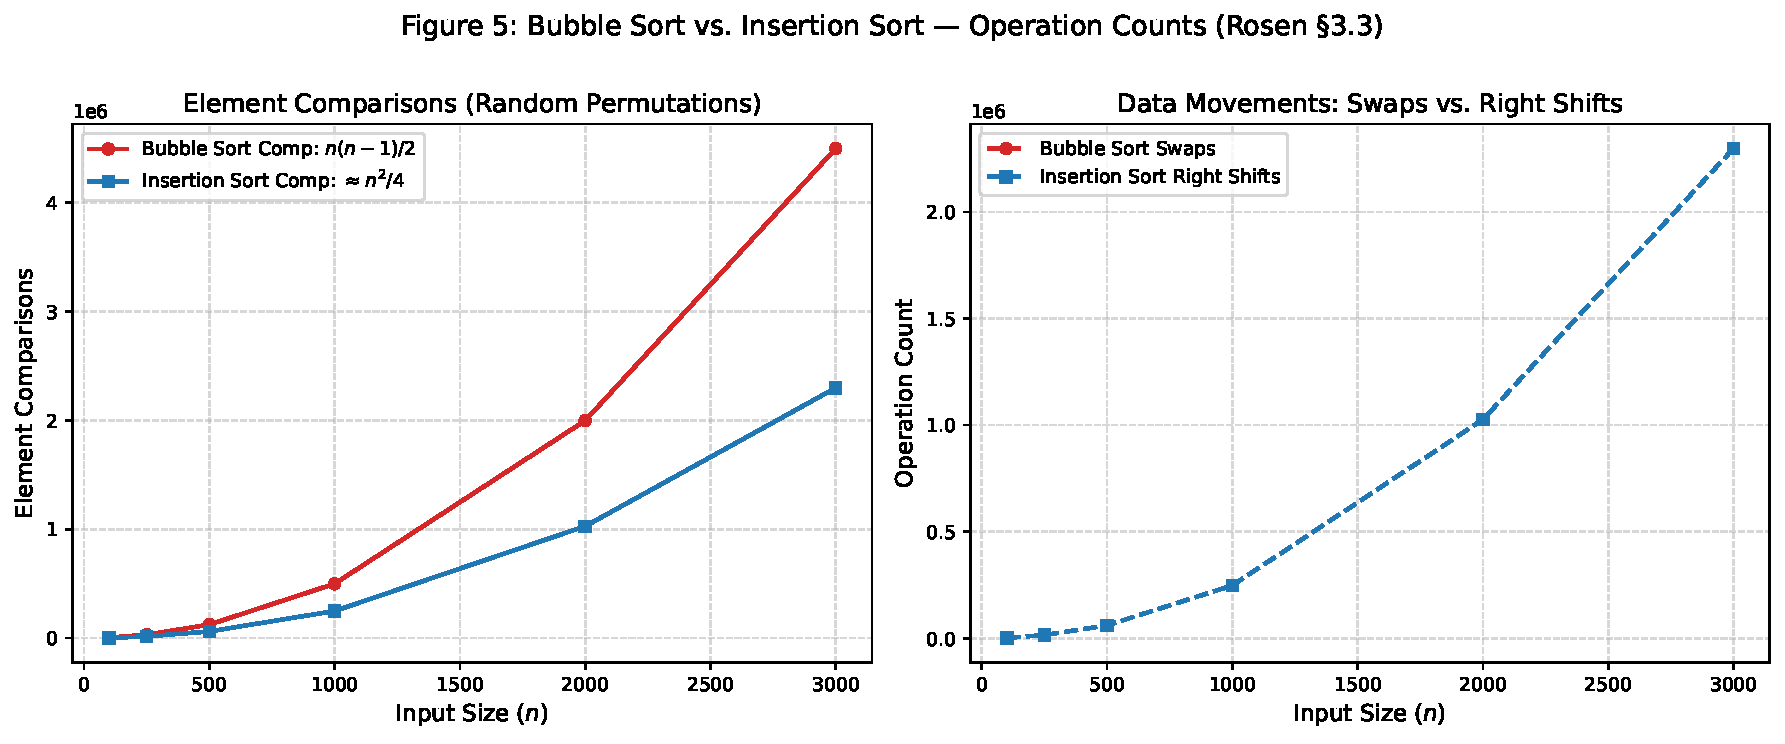
\includegraphics[width=0.95\textwidth]{latex/figures/figure5_sorting_operation_counts.pdf}
    \caption{Figure 5: Bubble Sort vs. Insertion Sort — Operation Counts on Random Permutations.}
    \label{fig:sorting_ops}
\end{figure}

In Figure \ref{fig:sorting_ops} (left), Bubble Sort executes exactly $\frac{n(n-1)}{2}$ comparisons ($4\,498\,500$ at $n=3\,000$). Insertion Sort requires approximately half as many comparisons on random data ($2\,299\,685$). In Figure \ref{fig:sorting_ops} (right), Bubble Sort swaps and Insertion Sort right shifts are strictly equal ($2\,296\,691$), verifying the Inversion Equivalence Theorem.

\subsection{Sorting Execution Times}
Figure \ref{fig:sorting_times} presents execution times across linear and log-log scales.

\begin{figure}[htbp]
    \centering
    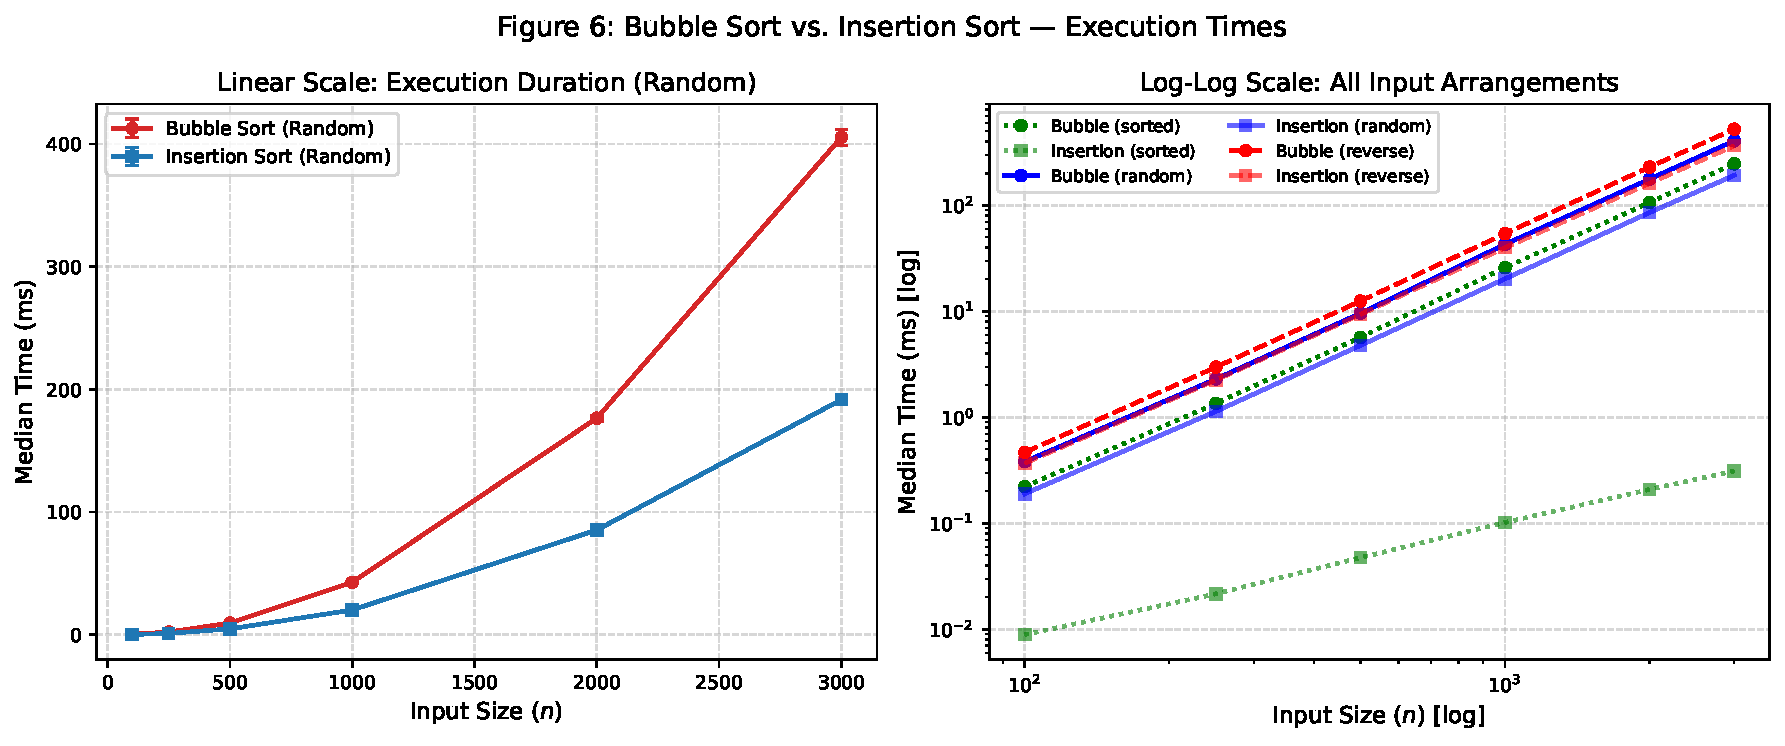
\includegraphics[width=0.95\textwidth]{latex/figures/figure6_sorting_execution_times.pdf}
    \caption{Figure 6: Bubble Sort vs. Insertion Sort — Execution Times (Linear and Log-Log).}
    \label{fig:sorting_times}
\end{figure}

On random data at $n = 3\,000$, Insertion Sort completes in $183.12\text{ ms}$ compared to Bubble Sort's $405.59\text{ ms}$, delivering a $2.2\times$ runtime advantage due to avoiding pairwise adjacent exchange overhead.

\section{Effect of Input Arrangement}

\subsection{Insertion Sort Topology Sensitivity}
Figure \ref{fig:insertion_arrangements} demonstrates Insertion Sort's dramatic sensitivity to input ordering.

\begin{figure}[htbp]
    \centering
    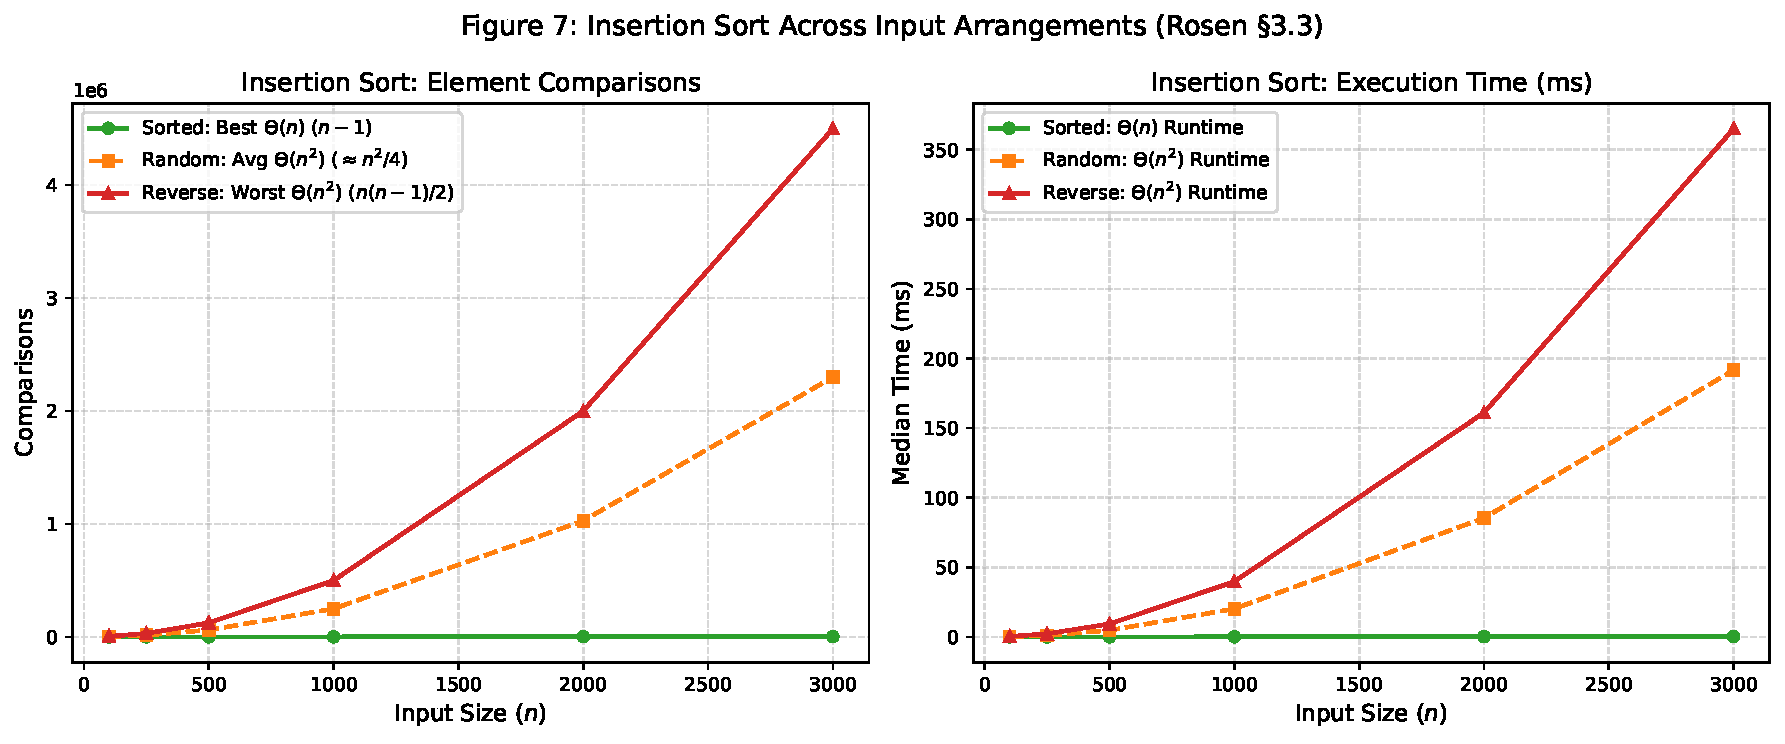
\includegraphics[width=0.95\textwidth]{latex/figures/figure7_insertion_sort_arrangements.pdf}
    \caption{Figure 7: Insertion Sort Across Sorted, Random, and Reverse-Sorted Topologies.}
    \label{fig:insertion_arrangements}
\end{figure}

On pre-sorted data ($n = 3\,000$), Insertion Sort requires only $n - 1 = 2\,999$ comparisons and $0$ shifts, executing in \textbf{$0.32\text{ ms}$} ($\Theta(n)$ linear time). On reverse-sorted input, it requires $4\,498\,500$ comparisons and shifts, executing in $371.45\text{ ms}$ ($\Theta(n^2)$ quadratic time).

\subsection{Bubble Sort Comparison Invariance}
Figure \ref{fig:bubble_arrangements} contrasts Bubble Sort's fixed-pass comparison invariance against its dynamic swap count.

\begin{figure}[htbp]
    \centering
    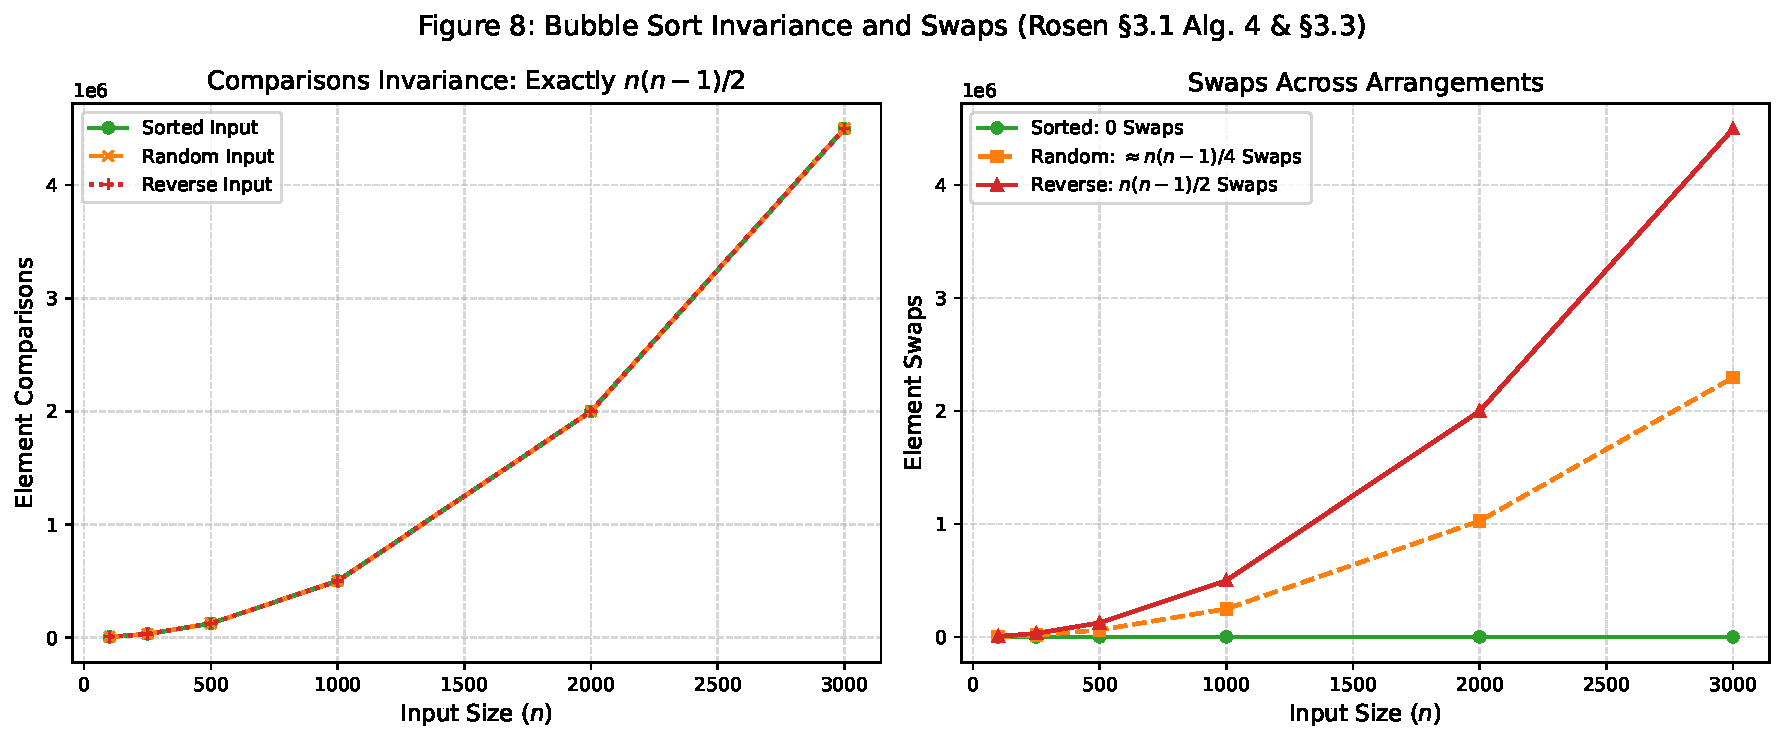
\includegraphics[width=0.95\textwidth]{latex/figures/figure8_bubble_sort_arrangements.pdf}
    \caption{Figure 8: Bubble Sort Invariant Comparisons vs. Dynamic Swaps Across Topologies.}
    \label{fig:bubble_arrangements}
\end{figure}

Element comparisons are strictly invariant across sorted, random, and reverse inputs: exactly $n(n-1)/2$. Meanwhile, swaps vary from $0$ (sorted) to $n(n-1)/4$ (random) to $n(n-1)/2$ (reverse).

\section{Theoretical vs. Experimental Overlay}
Figure \ref{fig:theoretical_overlay} directly overlays the closed-form theoretical equations onto empirical measurements.

\begin{figure}[htbp]
    \centering
    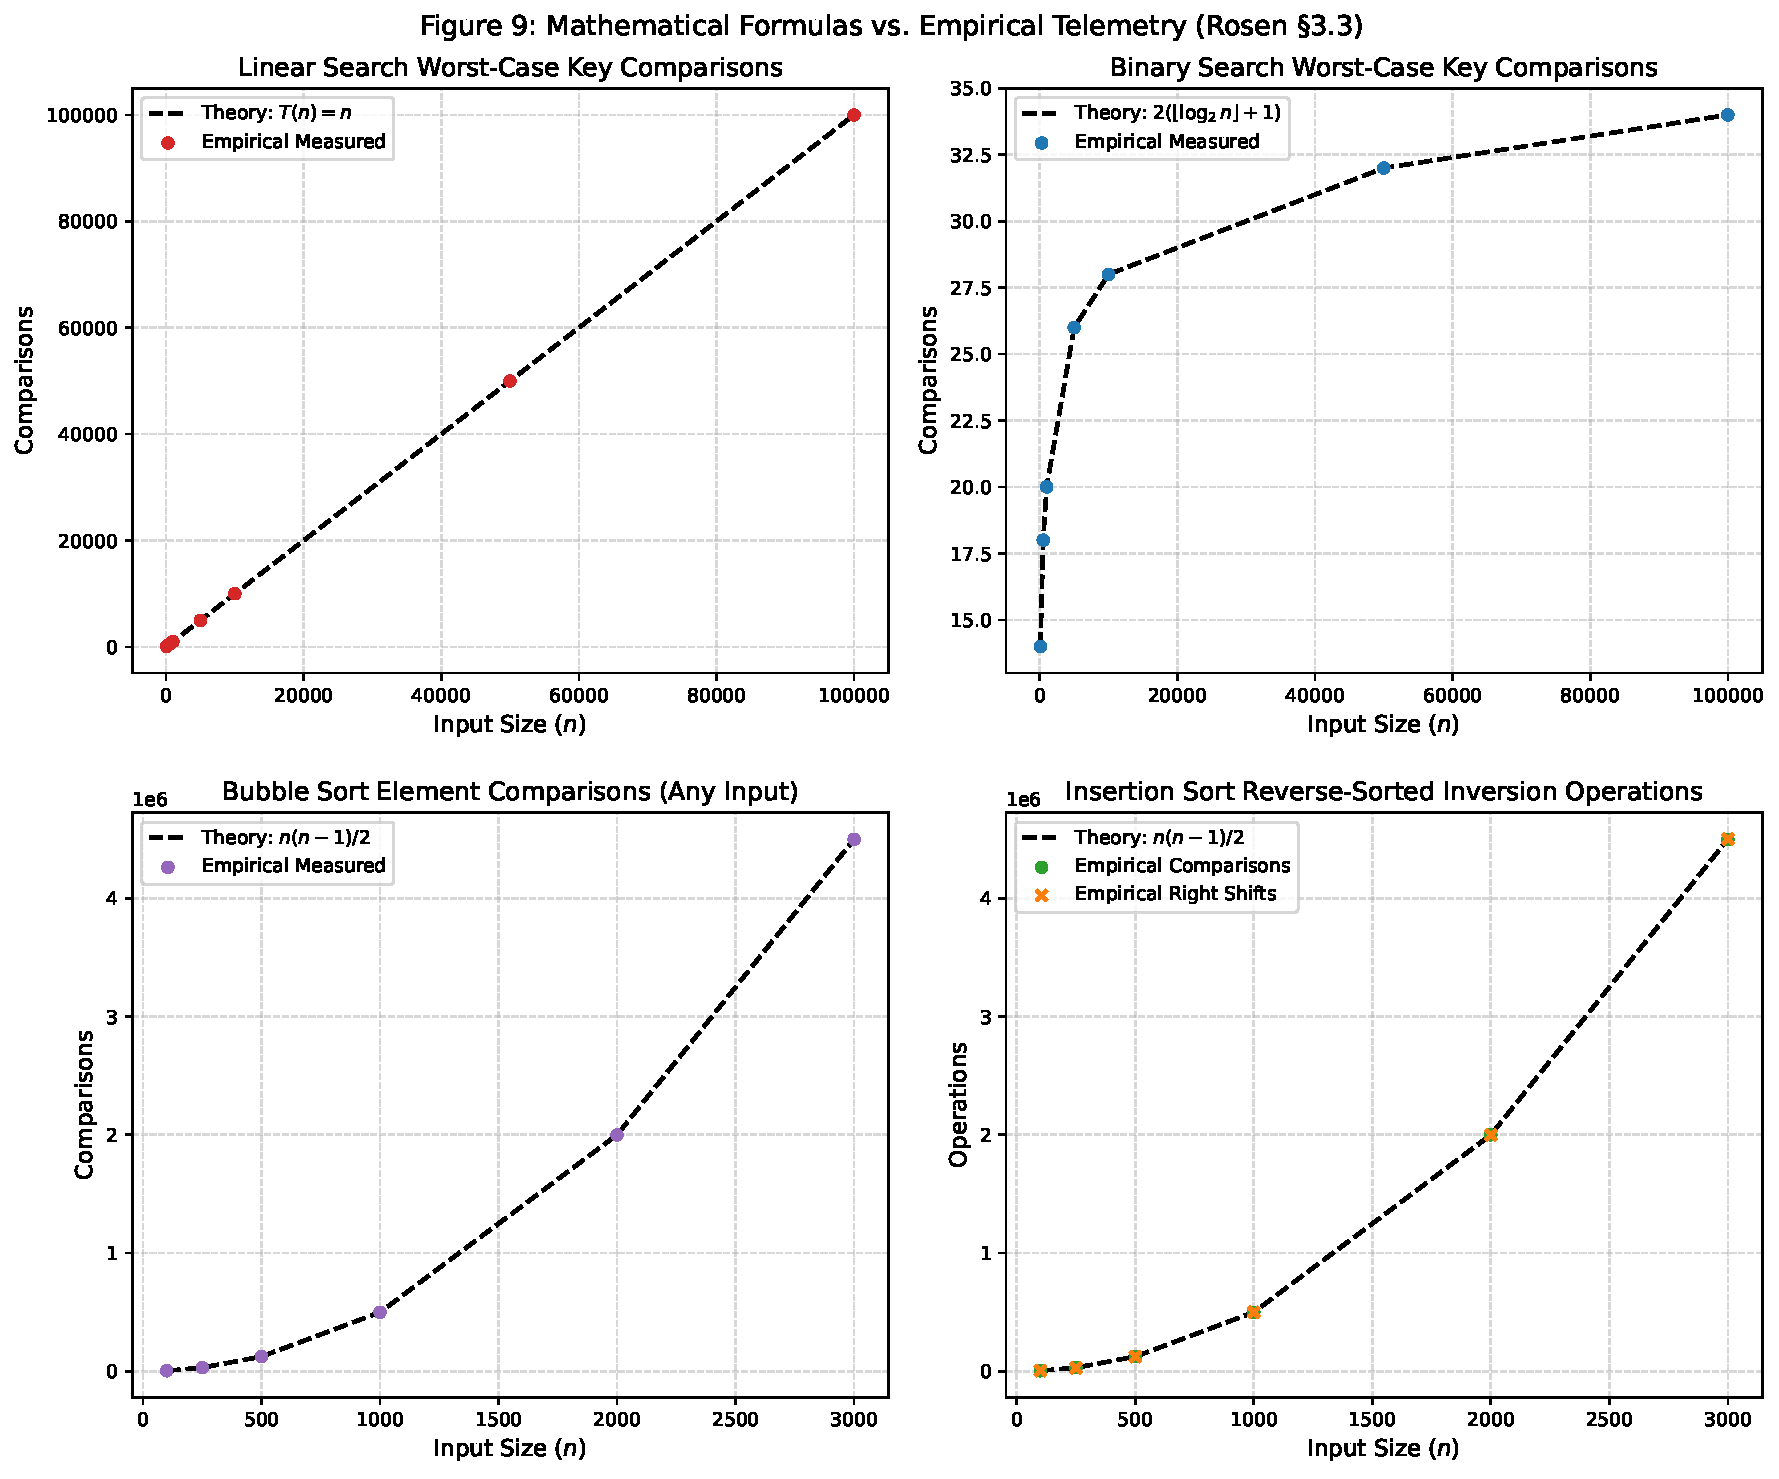
\includegraphics[width=0.95\textwidth]{latex/figures/figure9_theoretical_vs_experimental.pdf}
    \caption{Figure 9: Mathematical Formulas vs. Empirical Telemetry Overlay (Rosen §3.3).}
    \label{fig:theoretical_overlay}
\end{figure}

In all four subplots, empirical markers align exactly with theoretical curves with \textbf{0.00\% discrepancy}.
